\documentclass{article}
\usepackage{graphicx, mathtools, amsmath, amssymb, dirtytalk,float}

\graphicspath{{Images/}}

\setlength{\oddsidemargin}{0in}
\setlength{\textwidth}{6.5in}
\setlength{\topmargin}{-.55in}
\setlength{\textheight}{9in}
\pagestyle{empty}



\title{Scientific Computation II Final Exam}
\author{Michael Nameika}
\date{May 2023}

\begin{document}

\maketitle

\section*{Exercise 1: Application of RBF Interpolation - 2D reconstruction from a point cloud}
See HW4.

\section*{Exercise 2: 2D and 3D reconstruction from a point cloud}
\begin{itemize}
    \item[(a)] Modify the RBF interpolation to include a polynomial correction. In 2D, this amounts to searching the interpolant in the form
    \[F(\mathbf{x}) = \sum_{j = 1}^N c_j\phi(\|\mathbf{x} - \mathbf{x}_j\|) + p(x)\]
    where $p(\mathbf{x}) = p(x,y) = \gamma_1 + \gamma_2x + \gamma_3y$. [See Fornberg (2016) Part 1 for details ]
    \newline\newline
    Implementing the polynomial correction in 2D, our problem becomes one of solving for $M + 3$ coefficients, the $M$ coefficients as in exercise 1 plus $\gamma_1$, $\gamma_2$, and $\gamma_3$. We also require 
    \[\sum_{i = 1}^M c_i = \sum_{i=1}^M c_ix_i = \sum_{i=1}^M c_iy_i = 0.\]
    And so our linear system then becomes
    \[\begin{bmatrix}
         & & & | & 1 & x_1 & y_1\\
         & \phi(\|x_i - x_j\|) & & | & \vdots & \vdots & \vdots\\
         & & & | & 1 & x_M & y_M\\
         - & - & - & + & - & - & -\\
         1 & \cdots & 1 & | & 0 & 0 & 0\\
         x_1 & \cdots & x_M & | & 0 & 0 & 0\\
         y_1 & \cdots & y_M & | & 0 & 0 & 0
    \end{bmatrix}\begin{bmatrix}
        c_1\\
        \vdots\\
        c_M\\
        -\\
        \gamma_1\\
        \gamma_2\\
        \gamma_3
    \end{bmatrix} = \begin{bmatrix}
        0\\
        -\\
        \alpha\\
        -\\
        -\alpha\\
        -\\
        0\\
        0\\
        0
    \end{bmatrix}\]
    Modifying the script from exercise 1, we find the following plots using the polynomial correction:
    \begin{figure}[H]
        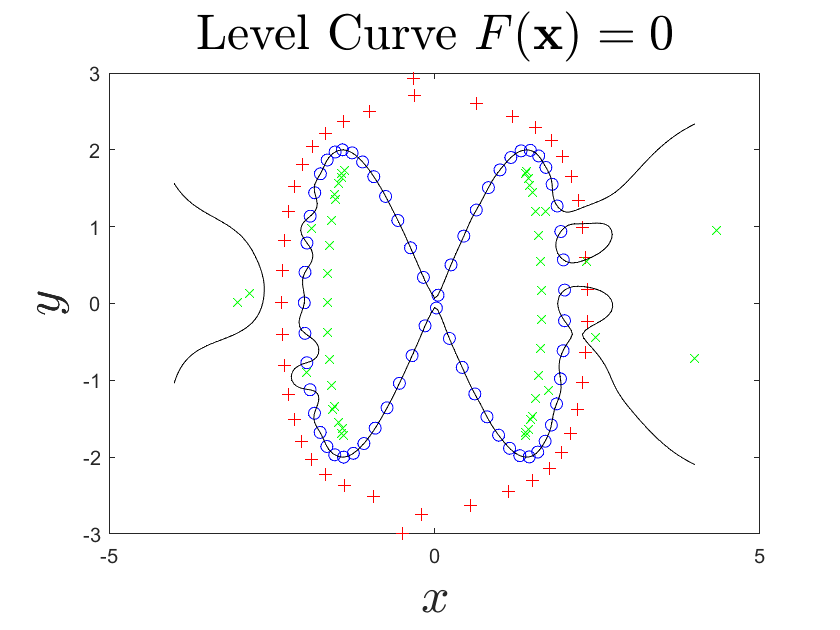
\includegraphics[scale = 0.4]{infinity_interp_poly.png}
        \centering
        \caption{Infinity Lissajous point cloud with polynomial correction $(\alpha = 0.1)$}
    \end{figure}
    \begin{figure}[H]
        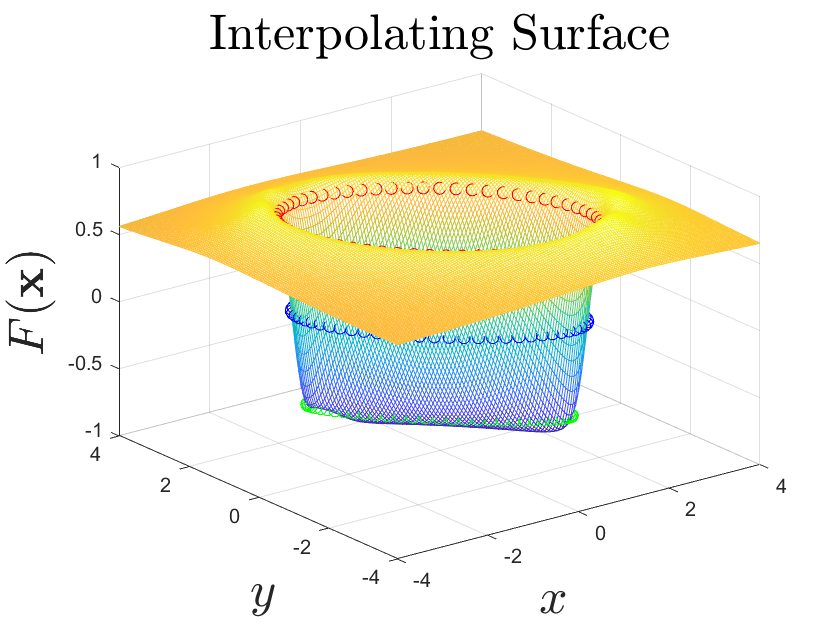
\includegraphics[scale = 0.35]{interpSurf_skewed_poly.png}
        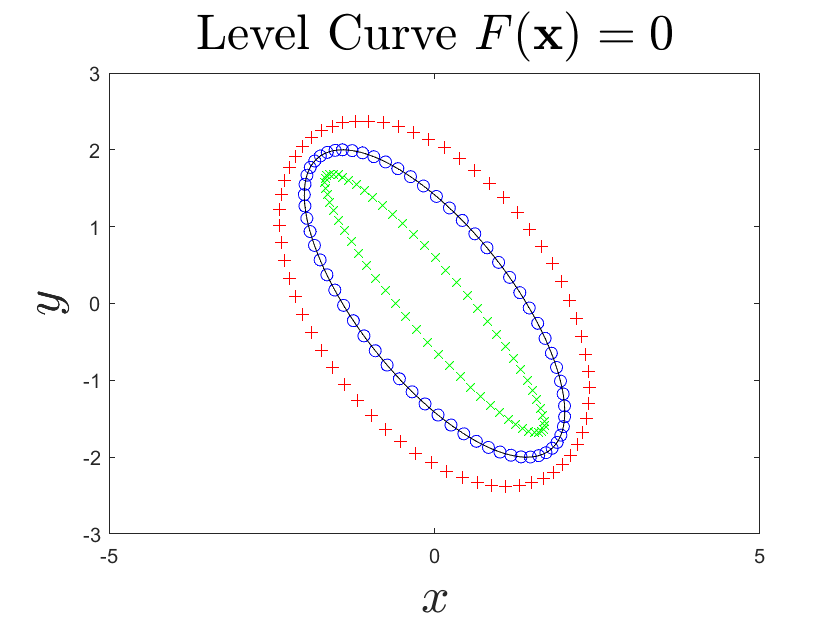
\includegraphics[scale = 0.35]{levelCurve_skewed_ploy.png}
        \centering
        \caption{"Skewed" ellipse point cloud with polynomial correction ($\alpha = 0.7$)}
    \end{figure}
    \begin{figure}[H]
        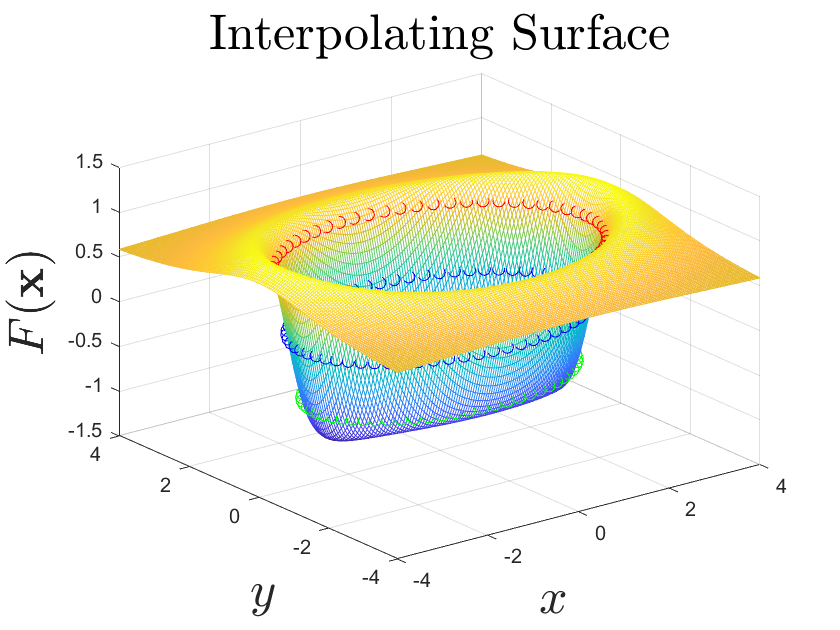
\includegraphics[scale = 0.35]{interpSurf_ellipse_poly.png}
        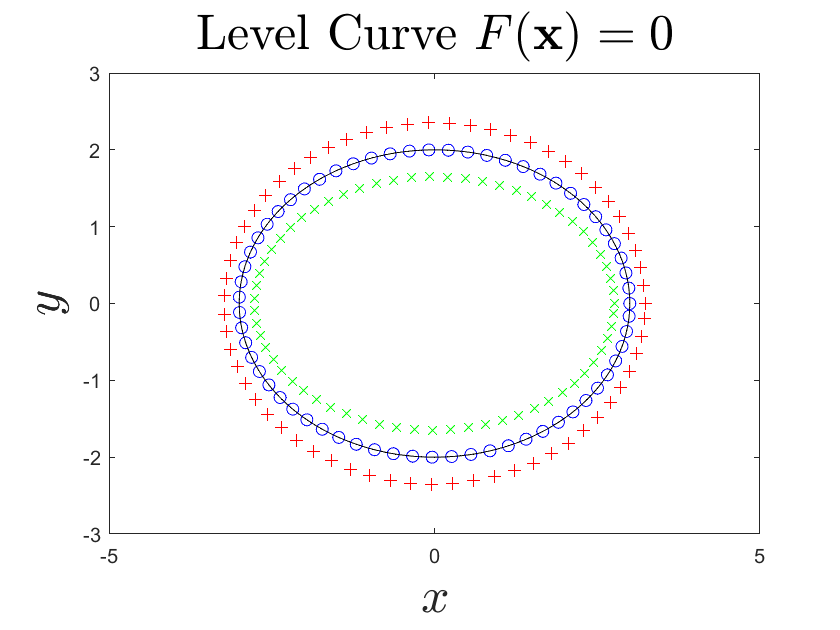
\includegraphics[scale = 0.35]{levelCurve_ellipse_poly.png}
        \centering
        \caption{Ellipse point cloud with polynomial correction ($\alpha = 0.4$)}
    \end{figure}
    
    

    \item[(b)] Solve the analogous problem in 3D, stating that given a 3D point cloud, find an implicit surface that approximates these $N$ points using RBF interpolants.
    \newline\newline
    Modifying the script from exercise 1 for a 3D implementation, we change the computation of the outward normal at a point $x_j$ to include any point within a predefined radius around $x_j$ and using the built-in \verb+isosurface+ command in \verb+MATLAB+ to plot a level surface, we find the following plots for an interpolation of a spherical point cloud of radius one in 3D (the spherical point cloud was generated by a parameterization of a sphere. See the attached \verb+my3DPointCloudRBF.m+ script for additional details.):
    \begin{figure}[H]
        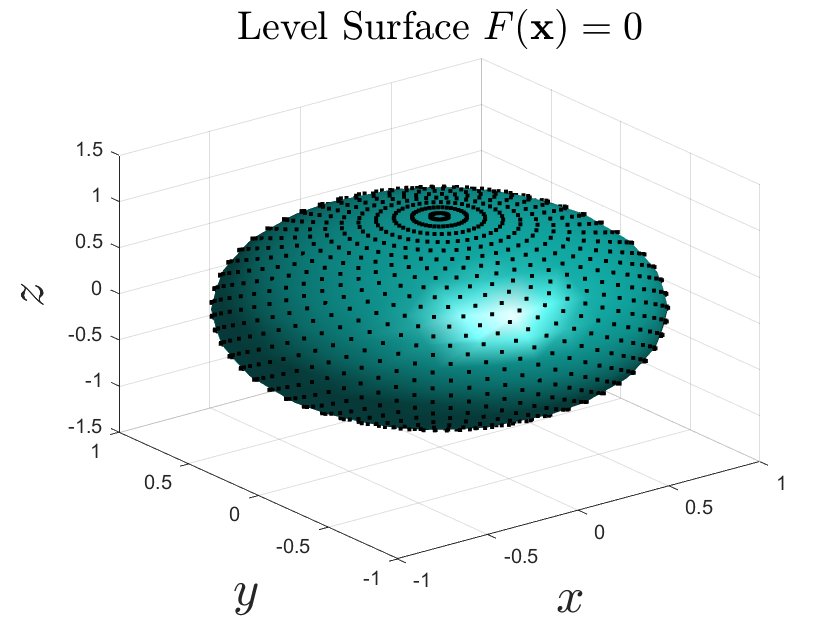
\includegraphics[scale = 0.5]{levelSphere_0_IMQ.png}
        \centering
        \caption{Level surface $F(x) = 0$ of interpolating function utilizing the IMQ RBF. Black dots are of the $x^0$ point cloud.}
    \end{figure}
    \begin{figure}[H]
        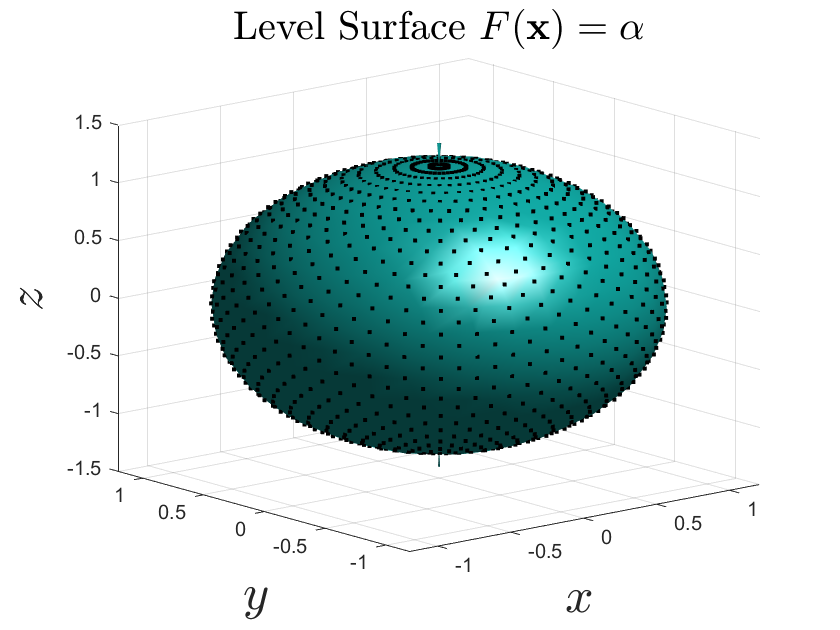
\includegraphics[scale = 0.5]{levelSphere_alpha_IMQ}
        \centering
        \caption{Level surface $F(x) = \alpha$ of interpolating function utilizing IMQ RBFs. Black dots are of the $x^+$ point cloud.}
    \end{figure}
    \begin{figure}[H]
        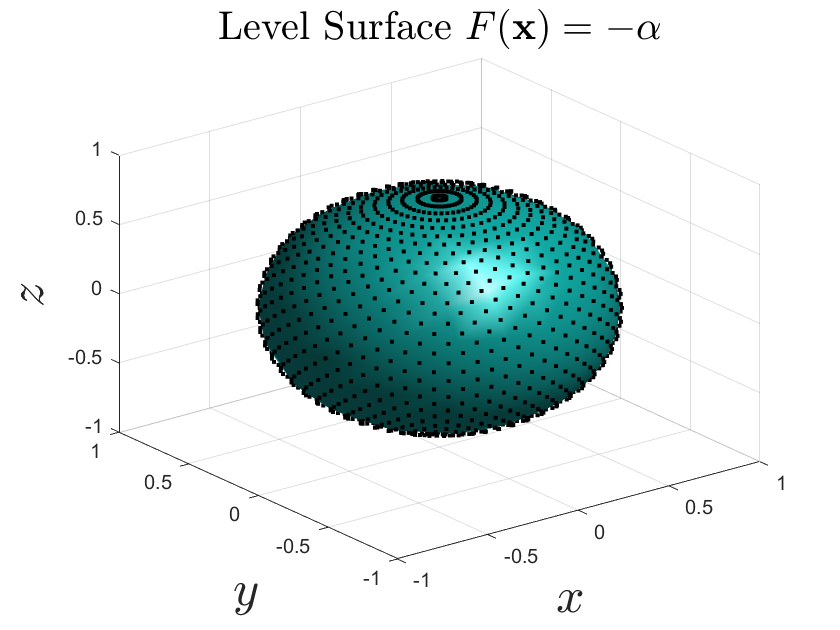
\includegraphics[scale = 0.5]{levelSphere_mAlpha_IMQ.png}
        \centering
        \caption{Level surface $F(x) = -\alpha$ of interpolating function utilizing IMQ RBFs. Black dots are of the $x^-$ point cloud.}
    \end{figure}
    
\end{itemize}

\section*{Exercise 3: RBF using pseudo-spectral Method}
\begin{itemize}
    \item[(a)] Apply the RBF-PS method to solve the heat equation and Helmholtz equation (eigenvalue problem for the Laplacian) in 1D. (The relevant material is Chapter 42-43 in Fasshauer).
    \newline\newline
    For the heat equation implementation, we seek to solve
    \[u_t = u_{xx}\]
    on the domain $x \in [0,1]$ with initial and boundary conditions
    \[u(x,0) = e^{-80x^2}; \hspace{1.2em} u(1,t) = u(0,t) = 0\]
    Approximating the function $u$ as a finite series of a radial basis function $\phi(x)$ yields
    \[\begin{bmatrix}
        & & &\\
        & \phi(\|x_i - x_j\|) & \\
        & & & 
    \end{bmatrix}\begin{bmatrix}
        c_1\\
        \vdots\\
        c_n
    \end{bmatrix} = \begin{bmatrix}
        u_1\\
        \vdots\\
        u_n
    \end{bmatrix}\]
    and so
    \[\begin{bmatrix}
         & & &\\
         & \phi''(\|x_i - x_j\|) & \\
          & & &
    \end{bmatrix}\begin{bmatrix}
        c_1\\
        \vdots\\
        c_n
    \end{bmatrix} = \begin{bmatrix}
        u''_1\\
        \vdots\\
        u''_n
    \end{bmatrix}\]
    For this problem, the inverse multiquadric RBF was utilized:
    \[\phi(x) = \frac{1}{\sqrt{1 + (\epsilon x)^2}}.\]
    With Euler time stepping:
    \[u_t(x_n,t_n) \approx \frac{u(x_n,t_n) - u(x_n,t_{n-1})}{dt}.\]
    Implementing this in \verb+MATLAB+ (see attached \verb+heateqRBF.m+ script), we find the following solution plot for $t \in [0, 1]$:
    \begin{center}
        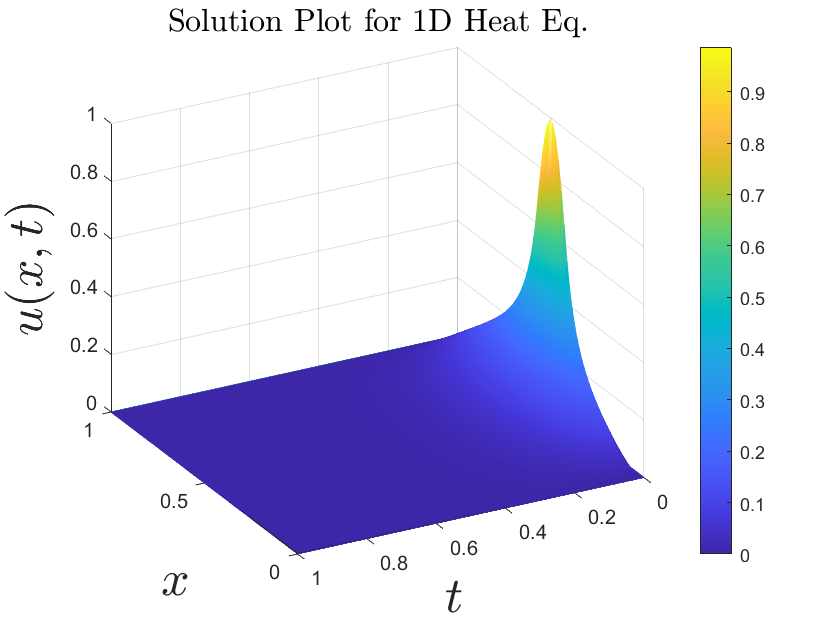
\includegraphics[scale = 0.5]{heatEqRBFSol}
    \end{center}
    Now, for the 1D Helmoltz eigenvalue problem, we wish to solve the eigenvalue problem
    \[\frac{d^2u}{dx^2} = \lambda u\]
    Solving analytically yields the eigenvalues
    \[\lambda_n = -n^2\pi^2, \hspace{0.5em} n \in \mathbb{N}\]
    and eigenfunctions
    \[u_n(x) = \sin(\sqrt{|\lambda_n|}x)\]
    Using the differentiation matrix we found to solve the heat equation (and the built-in \verb+MATLAB+ \verb+eig+ command), we find the the following eigenvalues and eigenfunctions:
    \begin{center}
        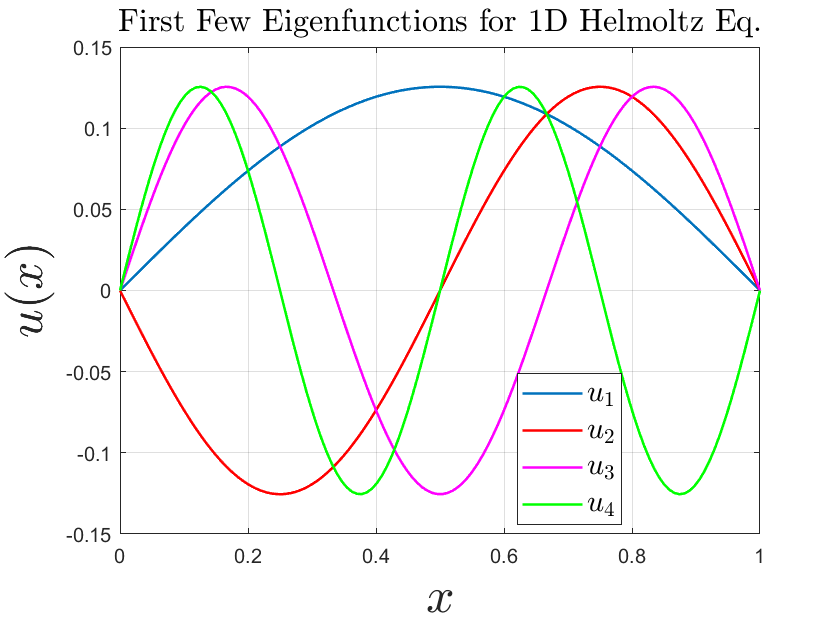
\includegraphics[scale = 0.5]{helmoltzEigFunc.png}
        \newline
        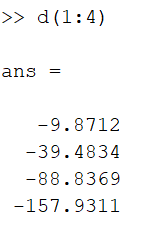
\includegraphics{helmholtzeig.png}
    \end{center}
    And an associated error plot for the first eigenfunction as we vary the number of spacial points $N$:
    \begin{center}
        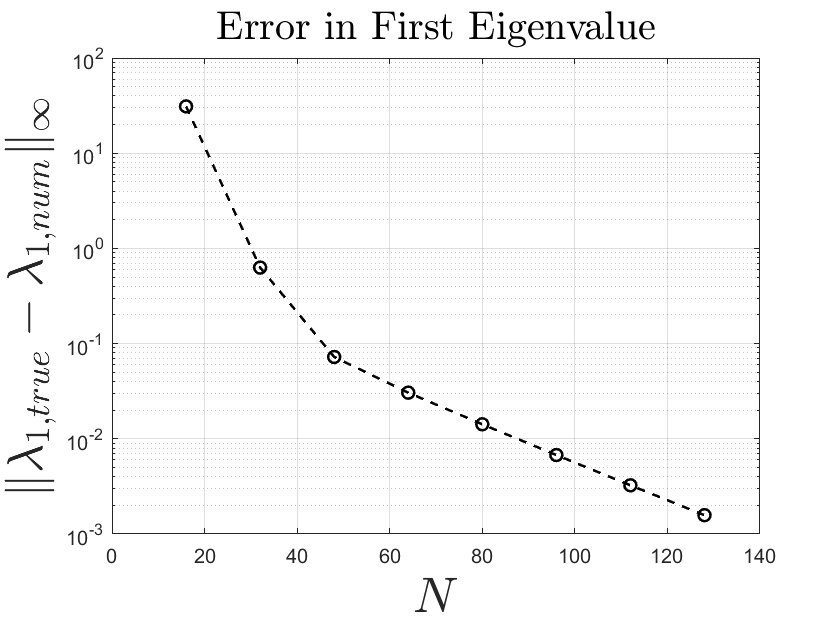
\includegraphics[scale = 0.5]{helmholtzeigerror.png}
    \end{center}
    

    \item[(b)] Describe the RBF-PS method in 2D (the implementation is optional).
    \newline\newline
    For this problem, we will consider the 2D heat equation and the 2D wave equation. Recall that the 2D heat equation takes the form
    \[u_t = k\nabla^2u\]
    with $\nabla^2$ denoting the Laplacian operator. And the wave equation takes the form
    \[u_{tt} = c^2\nabla^2u\]
    where $c$ is the wave speed. For our implementation, we will take $k = 1/32$ and $c = 1$. 
    For both equations, we will use Gaussian initial conditions with homogeneous Dirichlet boundary conditions. In particular, for the heat equation, we used the initial condition
    \[u(x,y,0) = e^{-40((x - 1/2)^2 + (y - 1/2)^2)}\]
    with $x \in [0, 1]$ and $y \in [0, 1]$.
    \newline
    To extend to 2D, our function $u(x,t)$ will be stored in an $N \times N$ matrix with the rows storing the $x$ values and the columns storing the $y$ values. To utilize matrix multiplication to approximate the derivative, we reshape the $u$ matrix to be $N^2 \times 1$. Then given the second derivative RBF differentiation matrix, our Laplacian operator matrix will be computed by
    \[L = D2 \otimes I + I \otimes D2\]
    with $I$ being an $N \times N$ identity matrix, and $\otimes$ denoting the Kronecker product. Implementing this in \verb+MATLAB+ (along with Euler time stepping), we find the following solution plots for heat equation for selected time values:
    \begin{center}
        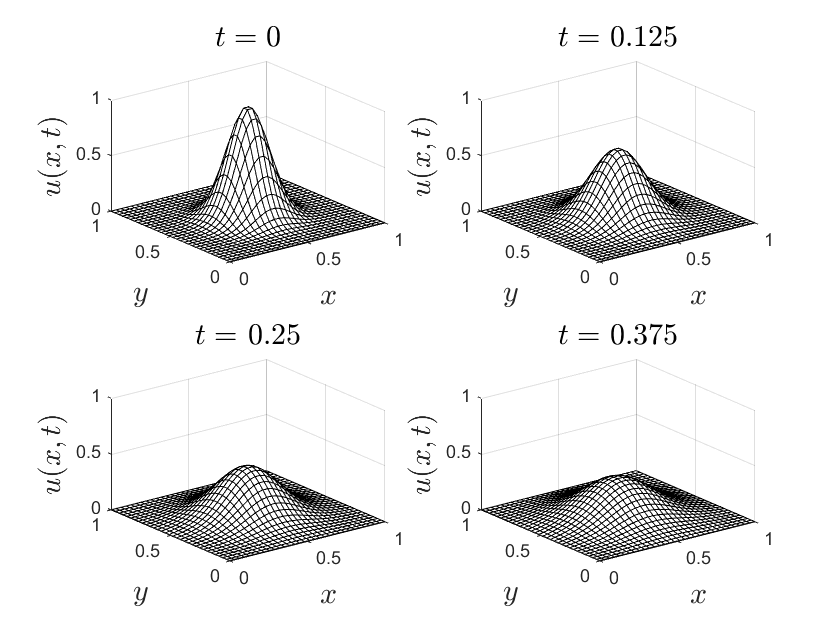
\includegraphics[scale = 0.5]{2D_heateq_RBF.png}
    \end{center}
    Now, for the wave equation, we use the initial condition 
    \[u(x,y,0) = e^{-40((x - 1/2)^2 + y^2)}\]
    with $x \in [-1, 1]$ and $y \in [-1,1]$.
    \newline
    Implementing into \verb+MATLAB+ (along with the second order approximation $u_{tt} \approx \frac{u(x,y,t_{n+1}) - 2u(x,y,t_n) + u(x,y,t_{n-1})}{\Delta t^2}$), we find the following solution plots for selected time values:
    \begin{center}
        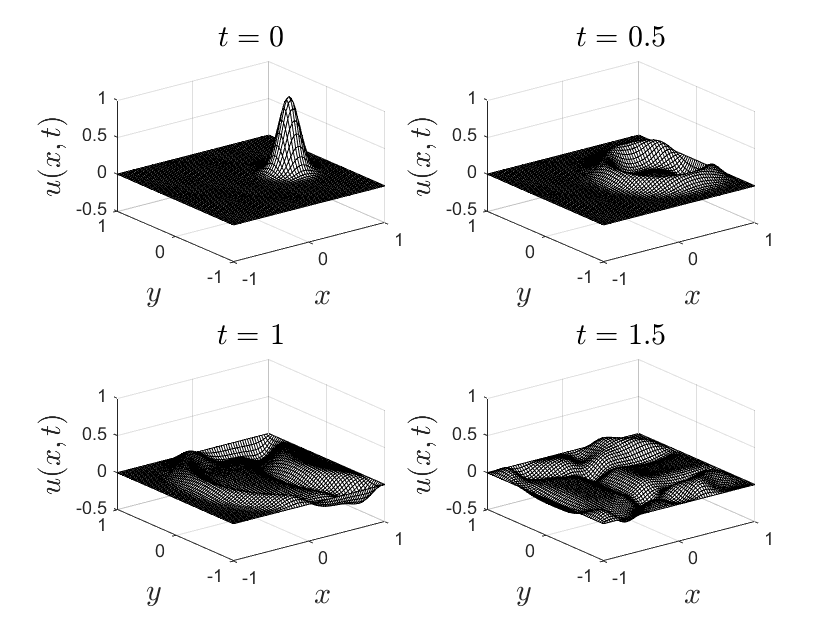
\includegraphics[scale = 0.5]{waveEq_RBF_PS.png}
    \end{center}
    For additional details, see the attached \verb+twoDheatEqRBFTest.m+ and \verb+twoDwaveEqTestRBF.m+ files.
\end{itemize}
\end{document}
